\documentclass[Ex4_Zusammenfassung.tex]{subfiles}

\begin{document}

\chapter{ Ex4 - Atomphysik}

In der Ex4-Vorlesung wird es um folgende Themen gehen:

\begin{itemize}
\item Atome
\item Kerne und Elementarteilchen
\item Symmetrien
\item schwache und starke Wechselwirkung
\item Spaltung und Fusion 
\end{itemize}
Johanna Stachels Notation: 
\begin{align*}
& e^2 = \frac{q_e^2}{4\pi \epsilon_{0}}  \\
& 1 \ eV = 1.60 \cdot 10^{-19} J  \\
& 1 \ fm = 10^{-15}  \ m \\ 
& 1 \ u = \  913 \ \nicefrac{MeV}{c^2} = 1.66 \cdot 10^{-27} kg \\
& \hslash = 6.58 \cdot 10^{-16} eVs = 1.05 \cdot 10^{-34} Js \\
&\alpha = \frac {e^2}{c \hslash} = \frac{1}{137} \\
&c = 3 \cdot 10^8 \  \nicefrac{m}{s} \\
\end{align*} \newpage

\section{Spektroskopische Notation}
Um den Zustand einer Unterschale nl anzugeben, führen wir die spektroskopische Notation ein: 
\begin{equation}
\centering \boxed{ n \ ^{2S+1}L_J }
\end{equation}
mit
\begin{align*}
&L := \sqrt{\frac{|\vec L|^2}{\hslash^2}- \frac{1}{4}} - \frac{1}{2} \in \frac{1}{2} \mathbb{N} \qquad \vec L:= \sum_{i} \vec l_i \\
&S :=  \sqrt{\frac{|\vec S|^2}{\hslash^2}- \frac{1}{4}} - \frac{1}{2} \in \frac{1}{2} \mathbb{N}  \qquad \vec S:= \sum_{i} \vec s_i \\
&J :=  \sqrt{\frac{|\vec L + \vec S |^2}{\hslash^2}- \frac{1}{4}} - \frac{1}{2} \in \frac{1}{2} \mathbb{N} \qquad \vec J:= \sum_{i} \vec j_i \\
\end{align*}
\newline
Die Notation für die Elemente des Periodensystems lautet: 
\begin{equation}
\centering \boxed{^{\qquad Massenzahl \  \frac{m}{u} } _{Kernladungszahl \  Z} \  El ^{\ \frac{q}{q_e} \  Ionisierung}} 
\end{equation}
\section{Hund'sche Regeln und Auswahlregeln}
Die Elektronen werden für die Grundzustände so aufgefüllt, dass die Bindungsenergie(negativ) minimiert wird, das heißt deren Betrag maximal wird. Zwischen den Unterschalen gilt folgende Reihenfolge: 
	\begin{figure}[H]
	\centering
	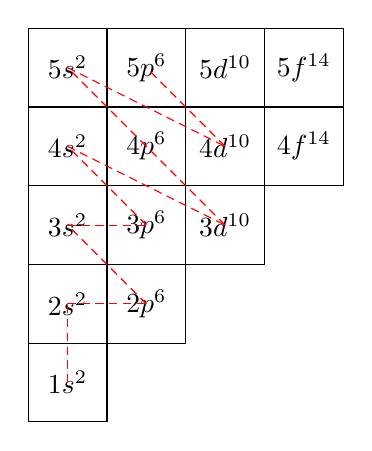
\begin{tikzpicture}
	\draw (0,0) +(-.5,-.5) rectangle ++(.5,.5);
	\draw (0,0) node{$1s^2$};
	\draw (0,1) +(-.5,-.5) rectangle ++(.5,.5);
	\draw (0,1) node{$2s^2$};
	\draw (0,2) +(-.5,-.5) rectangle ++(.5,.5);
	\draw (0,2) node{$3s^2$};
	\draw (0,3) +(-.5,-.5) rectangle ++(.5,.5);
	\draw (0,3) node{$4s^2$};
	\draw (0,4) +(-.5,-.5) rectangle ++(.5,.5);
	\draw (0,4) node{$5s^2$};

	\draw (1,1) +(-.5,-.5) rectangle ++(.5,.5);
	\draw (1,1) node{$2p^6$};
	\draw (1,2) +(-.5,-.5) rectangle ++(.5,.5);
	\draw (1,2) node{$3p^6$};
	\draw (1,3) +(-.5,-.5) rectangle ++(.5,.5);
	\draw (1,3) node{$4p^6$};
	\draw (1,4) +(-.5,-.5) rectangle ++(.5,.5);
	\draw (1,4) node{$5p^6$};

	\draw (2,2) +(-.5,-.5) rectangle ++(.5,.5);
	\draw (2,2) node{$3d^{10}$};
	\draw (2,3) +(-.5,-.5) rectangle ++(.5,.5);
	\draw (2,3) node{$4d^{10}$};
	\draw (2,4) +(-.5,-.5) rectangle ++(.5,.5);
	\draw (2,4) node{$5d^{10}$};

	\draw (3,3) +(-.5,-.5) rectangle ++(.5,.5);
	\draw (3,3) node{$4f^{14}$};
	\draw (3,4) +(-.5,-.5) rectangle ++(.5,.5);
	\draw (3,4) node{$5f^{14}$};

	\draw [draw = red, densely dashed] (0,0) -- (0,1);
	\draw [draw = red, densely dashed] (0,1) -- (1,1);
	\draw [draw = red, densely dashed] (1,1) -- (0,2);
	\draw [draw = red, densely dashed] (0,2) -- (1,2);
	\draw [draw = red, densely dashed] (1,2) -- (0,3);
	\draw [draw = red, densely dashed] (0,3) -- (2,2);
	\draw [draw = red, densely dashed] (2,2) -- (1,3);
	\draw [draw = red, densely dashed] (1,3) -- (0,4);
	\draw [draw = red, densely dashed] (0,4) -- (2,3);
	\draw [draw = red, densely dashed] (2,3) -- (1,4);
	\end{tikzpicture}
	\caption{Auffüllung der Grundzustände}
	\end{figure}
	Pro Unterzustand hat man $ N_e = 2(2l+1) $ Elektronen. 
	Die Gesamtzahl der Elektronen in der n-ten Schale entspricht somit $ N_e = 2 \sum_{l}^{n-1} 2l+1 =   2n^2 $

Innerhalb einer Unterschale gelten für die Grundzustände die hierarchischen \newline \textbf{Hund'schen Regeln}: 
\begin{enumerate}
\item Der Gesamtspin wird maximal. Das heißt hier ist $S = |\sum_i m_{s,i}| \stackrel{!}{=}$ max. 
\item Der Gesamtdrehimpuls  wird maximal. Das heißt hier ist  $L = |\sum_i m_{l,i}| \stackrel{!}{=}$ max.
\item Ist die Unterschale bis zu (einschließlich) halb voll, so wird J minimal. Das heißt hier ist  $ J := \lvert M_L + M_S \rvert \stackrel{!}{=} \lvert L-S \rvert $ , bei mehr als halb vollen Unterschalen muss $ J \stackrel{!}{=} L+S $ sein. 
\end{enumerate} 

Diese Regeln bestimmen die Feinstruktur des Elements. Regt man das Element an, so gelten diese Regeln nicht mehr. Möchte man verschiedene Zustände ihrer Energie nach ordnen, so ermittelt man den Grundzustand und verletzt dann die Regeln von unten nach oben.
Die  Schalen-/Orbitalübergänge werden von den sog. \textbf{Auswahlregeln} beherrscht, die wohlgemerkt nicht hierarchisch sind. 
\begin{enumerate}
\item $ \Delta L \  \in $ \{-1,1\}  bei L-S-Kopplung
\item $ \Delta M_L \   \in  $ \{-1,0,1\}  
\item $ \Delta S =0 $ für leichte Atome
\item $\Delta J \  \in $  \{-1,0,1\}   wobei $ \ J =0 \  \rightarrow J=0 \  \textbf{verboten} $
\end{enumerate}

\section{Vielelektronenprobleme} 
Für Elemente mit mehr als einem Elektron gibt es keine analytische Lösung der Schrödinger-Gleichung, auch numerische Verfahren sind mit zunehmender Elektronenzahl extrem aufwändig. Wir machen deshalb folgende Näherungen:
\textbf{Alkaliatome (1.Hauptgruppe)} \newline 
\begin{itemize}
\item Alkaliatome haben nur ein Elektron außerhalb geschlossener Schalen. Die Grundzustände sind immer $ \ ^{2}S_{\frac{1}{2}} $ ( $ n  \in \{2,3,4,...\} $ nicht notiert).
\item Wir betrachten zu Näherung ein \textbf{effektives Potential} $ V_{eff}(r) $ \newline \newline
 $ V_{eff}(r) = - \frac{e^2 Z_{eff}(r)}{r} $ mit $ 1 < Z_{eff}(r) < Z $ \  und  $ Z_ {eff} \stackrel{r\rightarrow \infty}{\rightarrow} 1, \ Z_{eff} \stackrel{r \rightarrow 0}{\rightarrow} Z $
 
\begin{figure}[h]
\centering
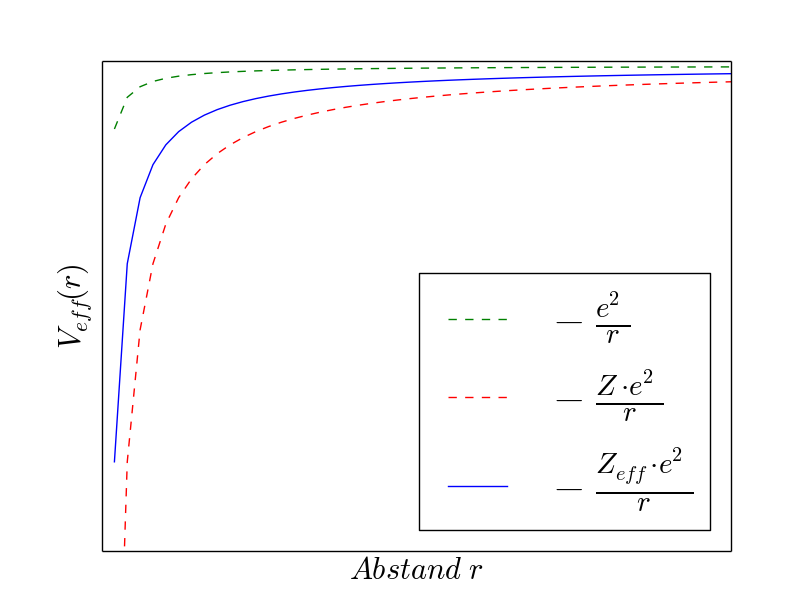
\includegraphics[height= 6cm, width=9cm]{effpot.png}
\caption{ Effektives Potential }
\end{figure}
 \item Dies hebt die $ E_n $ -Entartung bezüglich Z bereits auf (Feinstruktur): \newline
$ E_n(s) < E_n(p) < E_n(d) < E_n(f)$ (für kleine n am stärksten)
\item Für große n und r (wasserstoffähnlich) lässt sich dies so schreiben: 
 	\begin{equation}
 	E_{n,l} = -E_0 \frac{Z_{eff}^2}{n^2} = - \frac{E_0}{n_{eff}^2} = - \frac{E_0}{(n-\delta_{n,l})^2} 			\qquad E_0 = 13.6 \  eV 
 	\end{equation}
 wobei $\delta_{n,l} $ der sog. \textbf{Quantendefekt} ist: $ \delta_{n,l} = n - \sqrt{\frac{E_0}{-E_{n,l}}} \newline  E_{n,l} <\  0  $ ist die real gemessene Energie. 

\end{itemize}
Um allgemeine Vielelektronenprobleme zu lösen, können wir (zumindest bis jetzt) nur nähern indem wir zur Lösung eines Elektron die anderen Elektronen unabhängig voneinander gelöst haben und das entstehende $ V_{eff}(r) $ \textbf{kugelsymmetrisch} ist. \newline
Wir suchen deshalb eine  \textbf{Gesamtwellenfunktion für N Teilchen}. \newline
Diese muss antisymmetrisch unter Vertauschung sein, wir nehmen zusätzlich an, dass sie sich als Produkt der Einteilchenwellenfunktionen schreiben lässt. \newline 
Analog zu $ \psi_{ges}(1,2) = \psi_1(1) \psi_2(2) - \psi_2(1) \psi_1(2) $  definieren wir die \\ \textbf{Slaterdeterminante}: 
	\begin{equation}
	  \psi_{ges}(r_1,...,r_N) \ = \  \frac{1}{\sqrt{N!}} \  det \begin{pmatrix} \psi_1(1) & \psi_1(2) & \dots & \psi_1(N) \\ \vdots & \vdots & \vdots & \vdots \\  \psi_N(1) & \psi_N(2) & \dots & \psi_N(N)  \end{pmatrix} 
	\end{equation}
Diese ist total antisymmetrisch unter Spaltenvertauschung als Summe und N! Produkten. 
\section{Moseley'sches-Gesetz}
Für Eletronen-übergänge zwischen Zuständen wurde empirisch festgestellt, dass $ \sqrt{f} \propto Z $ ist, wobei f die Frequenz des emittiereten Lichts ist. 
\begin{align*}
\textbf{Moseley'sches Gesetz:} \ f \ &= \frac{E_0 (Z-b)^2}{h (1+\nicefrac{m_e}{M_{core}})} \left(\frac{1}{n_2^2} - \frac{1}{n_1^2}\right) \\ 
\lambda \ & = \frac{h(1+\nicefrac{m_e}{M_{core}})}{E_0 (Z-b)^2} \frac{1}{\nicefrac{1}{n_2^2} - \nicefrac{1}{n_1^2}} 
\end{align*}
für Übergänge $ n_1 \rightarrow n_2 $ , b - Abschirmkonstante \newline
Für das Wasserstoffatom entspricht das Moseley-Gesetz der Rydberg-Formel. \\ \newline
Für wasserstoffähnliche Atome gilt b=(Z-1) : \newline \quad K-Linien: $ n_2 = 1, \  K_{\alpha} :  n_1 = 2, \  K_{\beta}: n_1 = 3 $ \\ \newline
Für schwere Atome ($ Z > 40 $  )  gilt : \newline \qquad L-Linien: $ n_2 = 2 , b \approx 7.4 , \ L_{\alpha} : \ n_1= 3 , \  L_{\beta}: n_1 = 4 $ \\  \newline
Die Auswahlregeln müssen gelten. \newpage
\end{document}